\begin{name}
	{\tenchude}
	{\tendethi}
	{\tentruong}
	{\thoigian}
\end{name}
\caulc
\Opensolutionfile{ans}[ans/10-CK1-THCS-THPT-DienHong-Phan-1]
\begin{ex}%[1D3H1-2]%[Dự án tex đề HK1 năm học 2024-2025, Huỳnh Quy]
	Tính giới hạn dãy số $\lim \dfrac{2n+3}{n+1}$?
	\choice
	{$0$}
	{$3$}
	{$1$}
	{\True $2$}
	\loigiai{
		Ta có $\lim \dfrac{2n+3}{n+1}=\lim\dfrac{2+\dfrac{3}{n}}{1+\dfrac{1}{n}}=\dfrac{2}{1}=2$.
	}
\end{ex}
\begin{ex}%[1D2H2-4]%[Dự án tex đề HK1 năm học 2024-2025, Huỳnh Quy]
	Cho một cấp số cộng có $u_1=5$ và công sai $d=4$. Tìm số hạng thứ $100$ của cấp số cộng đó?
	\choice
	{$405$}
	{$400$}
	{$105$}
	{\True $401$}
	\loigiai{
		Ta có $u_{100}=u_1+99d=5+99\cdot 4=401$.
	}
\end{ex}
\begin{ex}%[BG K10-K11-LVH, Dat Tien Pham]%[1H4N1-1]
Một hình chóp có đáy là ngũ giác có số mặt và số cạnh là
\choice
{$6$ mặt, $5$ cạnh}
{\True $6$ mặt, $10$ cạnh}
{$5$ mặt, $10$ cạnh}
{$5$ mặt, $5$ cạnh}
\loigiai{
Hình chóp ngũ giác có $5$ mặt bên và $1$ mặt đáy, $5$ cạnh bên và $5$ cạnh đáy.
\begin{tikzpicture}[font=\footnotesize, line join=round, line cap=round,>=stealth, scale=.7]
\coordinate (A) at (0,0);
\coordinate (B) at (3,1.5);
\coordinate (D) at (4.5,-1.5);
\coordinate (C) at (6.5,0.5);
\coordinate (E) at (2,-2);
\coordinate (S) at (2.5,5);
\draw (S)--(A)(S)--(E) (S)--(D) (D)--(E) (E)--(A) (S)--(C) (C)--(D) (S)--(D);
\draw[dashed] (A)--(B) (B)--(C) (S)--(B);
%\tkzDrawSegments(S,A S,E S,D D,E E,A C,S C,D S,D)
%\tkzDrawSegments[dashed](A,B B,C S,B)
\foreach \x/\g in {A/180,B/-90,C/0,D/-90,E/-90,S/90}
\fill (\x) circle (1pt)
($(\x)+(\g:3mm)$) node{$\x$};
\end{tikzpicture}
}
\end{ex}
\begin{ex}%[1H4H2-3]%[Dự án tex đề HK1 năm học 2024-2025, Huỳnh Quy]
	\immini{Cho hình chóp $S. ABCD$ có đáy là hình thang đáy lớn $AD$. Gọi $M$, $N$ lần lượt là trung diểm của $SB$, $SD$. Giao tuyến của hai mặt phẳng $(AMN)$ và $(ABCD)$ là đường thẳng song song với
	\choice
	{Đường thẳng $AC$}
	{Đường thẳng $CD$}
	{Đường thẳng $AD$}
	{\True Đường thẳng $BD$}}{
	\begin{tikzpicture}[line cap=round,>=stealth]
		\coordinate (A) at (0,0);
		\coordinate (D) at (4,0);
		\coordinate (B) at (-1,-1);
		\coordinate (C) at (3,-1);
		\coordinate (S) at ($(A)+(0,3)$);
		\coordinate (M) at ($(S)!0.5!(B)$);
		\coordinate (N) at ($(S)!0.5!(D)$);
		\foreach \x in {A,B,C,D,S,M,N}{\draw[fill=black] (\x) circle (1pt);}
		\draw (S)--(B)--(C)--(D)--cycle;
		\draw (S)--(C);
		\draw[dashed] (A)--(B) (A)--(D) (S)--(A) (A)--(M)--(N)--cycle;
		\draw (S) node[above]{$S$};
		\draw (A) node[left]{$A$};
		\draw (B) node[below left]{$B$};
		\draw (C) node[below]{$C$};
		\draw (D) node[right]{$D$};
		\draw (M) node[left]{$M$};
		\draw (N) node[right]{$N$};
	\end{tikzpicture}
	}
	\loigiai{
		Ta có $A$ là một điểm chung của hai mặt phẳng $(AMN)$ và $(ABCD)$.\\
		Lại có $MN\parallel BD$ (Vì $MN$ là đường trung bình của tam giác $SBD$).\\
		Mà $MN\subset(AMN)$, $BD\subset(ABCD)$.\\
		Do đó $(AMN)\cap(ABCD)=Ax\parallel MN\parallel BD$.}
\end{ex}

\begin{ex}%[1D1H5-3]%[Dự án tex đề HK1 năm học 2024-2025, Huỳnh Quy]
	Tập nghiệm của phương trình $\sin x=-1$ là
	\choice
	{$x=\dfrac{\pi}{2}+k\pi$}
	{$x=-\dfrac{\pi}{4}+k2\pi$}
	{\True $x=-\dfrac{\pi}{2}+k2\pi$}
	{$x=-\dfrac{\pi}{2}+k\pi$}
	\loigiai{
		Ta có $\sin x=-1\Leftrightarrow x=-\dfrac{\pi}{2}+k2\pi$.
	}
\end{ex}

\begin{ex}%[1D2H1-3]%[Dự án tex đề HK1 năm học 2024-2025, Huỳnh Quy]
	Cho dãy số $(u_n)$ với $u_n=\dfrac{n+2}{2n+3}$, $n \in \mathbb{N}^{*}$. Tìm số hạng đầu tiên của dãy số $(u_n)$.
	\choice
	{$u_1=-\dfrac{2}{3}$}
	{$u_1=\dfrac{1}{9}$}
	{\True $u_1=\dfrac{3}{5}$}
	{$u_1=-\dfrac{1}{3}$}
	\loigiai{
		Ta có $u_1=\dfrac{1+2}{2\cdot 1+3}=\dfrac{3}{5}$.
	}
\end{ex}
\begin{ex}%[1D1H2-4]%[Dự án tex đề HK1 năm học 2024-2025, Huỳnh Quy]
	Chọn công thức sai trong các công thức sau?
	\choice
	{\True $\cos (2024\pi+x)=-\cos x$}
	{$\cos (\pi+x)=-\cos x$}
	{$\sin (\pi-x)=\sin x$}
	{$\cos \left(\dfrac{\pi}{2}-x\right)=\sin x$}
	\loigiai{
		Ta có $\cos (2024\pi+x)=\cos x$ là công thức sai.
	}
\end{ex}
\begin{ex}%[1D1N1-1]
Gọi $S$ là tập hợp các giả trị của $x$ trên đoạn $\left[-\pi ; \dfrac{3 \pi}{2}\right]$ để hàm số $y=\cos x$ nhận giá trị dương. Khi đó $S$ là tập hợp nào sau đây ?
\choice
{\True $\left(-\dfrac{\pi}{2} ; \dfrac{\pi}{2}\right)$}
{$\left[-\dfrac{\pi}{2} ; \dfrac{\pi}{2}\right]$}
{$\left[-\dfrac{\pi}{2} ; \pi\right]$}
{$(0 ; \pi)$}
\loigiai{Ta có đồ thị hàm số $y=\cos x$.\\
\begin{tikzpicture}
[>=stealth,x=1cm,y=1cm]
\draw[->,line width = 1pt] (-7.5,0)--(0,0)%
node[below right]{$O$}--(7.5,0) node[below]{$x$};
\draw (-1.8,0) node[above]{$-\dfrac{\pi}{2}$} (1.57,0) node[above]{$\dfrac{\pi}{2}$};
\draw[->,line width = 1pt] (0,-2) --(0,2) node[right]{$y$};
\draw (-3.14,0) node[above]{$-\pi$} (3.14,0) node[above]{$\pi$};
\draw (-4.71,0) node[above]{$-\dfrac{3\pi}{2}$} (4.6,0) node[above]{$\dfrac{3\pi}{2}$};
\draw (-6.28,0) node[below]{$-2\pi$} (6.28,0) node[above]{$2\pi$};
\foreach \y in {-1,1}{
\draw (0,\y) node[left]{$\y$} circle (1pt);%Oy
}
\draw [green!50!black, black, line width = 1.2pt, domain=-7.5:7.5, samples=100]%
plot (\x, {cos(\x*180/pi)}) node[right]{$y=\cos x$};
\draw [dashed] (-7.5,1)--(7.5,1);
\draw [dashed] (-7.5,-1)--(7.5,-1);
\draw [dashed] (-6.28,1)--(-6.28,0);
%\draw [dashed] (-4.71,1)--(-4.71,-1);
\draw [dashed] (-3.14,-1)--(-3.14,0);
%\draw [dashed] (-1.57,0)--(-1.57,-1);
%\draw [dashed] (1.57,1)--(1.57,-1);
\draw [dashed] (3.14,0)--(3.14,-1);
%\draw [dashed] (4.71,1)--(4.71,-1);
\draw [dashed] (6.28,0)--(6.28,-1);
\end{tikzpicture}\\
Từ đồ thị hàm số $y=\cos x$ trên đoạn $\left[- \pi ; \dfrac{3 \pi}{2}\right]$, ta thấy hàm số $y=\cos x$ nhận giá trị dương khi $x\in \left(\dfrac{- \pi}{2}; \dfrac{ \pi}{2}\right)$.\\
Vậy $S=\left(\dfrac{- \pi}{2}; \dfrac{ \pi}{2}\right)$.
}
\end{ex}
\begin{ex}%[1D1H4-2]%[Dự án tex đề HK1 năm học 2024-2025, Huỳnh Quy]
	Tập xác định của hàm số $y=\tan x$ là
	\choice
	{$\mathscr{D}=\mathbb{R} \setminus\{\pi+k \pi \mid k \in \mathbb{Z}\}$}
	{\True $\mathscr{D}=\mathbb{R} \setminus\left\{\dfrac{\pi}{2}+k \pi \mid k \in \mathbb{Z}\right\}$}
	{$\mathscr{D}=\mathbb{R} \setminus\{k \pi \mid k \in \mathbb{Z}\}$}
	{$\mathscr{D}=\mathbb{R} \setminus\{k 2\pi \mid k \in \mathbb{Z}\}$}
	\loigiai{
		Ta có $y=\tan x=\dfrac{\sin x}{\cos x}$.\\
		Điều kiện xác định: $\cos x\ne 0\Leftrightarrow x\ne \dfrac{\pi}{2}+k\pi$, $k\in\mathbb{Z}$.
	}
\end{ex}

\begin{ex}%[1D2N2-1]
Trong các dãy số sau, dãy số nào là một cấp số cộng?
\choice
{$ 1;-3;-5;-7;-9$}
{$ 1;-2;-4;-6;-8$}
{\True $ 1;-3;-7;-11;-15$}
{$ 1;-3;-6;-9;-12$}
\loigiai{
Dãy số $ 1;-3;-7;-11;-15$ là cấp số cộng với công sai $d=-4$	.
}
\end{ex}

\begin{ex}%[1D5N1-2]
Cho bảng số liệu khảo sát về tuổi thọ (đơn vị: nghìn giờ) của một loại bóng đèn:
\begin{longtable}{|c|c|c|c|c|c|}
\hline Tuổi thọ &{$[3 ; 5)$}&{$[5 ; 7)$}&{$[7 ; 9)$}&{$[9 ; 11)$}&{$[11 ; 13)$}\\
\hline Số bóng đèn & $4$ & $20$ & $26$ & $42$ & $8$ \\
\hline
\end{longtable}
Có bao nhiêu bóng đèn được khảo sát có tuổi thọ từ $9$ nghìn giờ trở lên?
\choice
{$24$}
{$24$}
{$42$}
{\True $50$}
\loigiai{
Số bóng đèn được khảo sát có tuổi thọ từ $9$ nghìn giờ trở lên là $42+8=50$.
}
\end{ex}

\begin{ex}%[1D5N2-2]%[Dự án 11 HVA 2024-2025]%[Bình Toán]
Khảo sát thời gian chạy bộ trong một ngày của một số học sinh khối 11 thu được mẫu số liệu ghép nhóm sau
\begin{center}
\begin{tabular}{|c|c|c|c|c|c|}
\hline
Thời gian (phút) & $[0 ; 20)$ & $[20 ; 40)$ & $[40 ; 60)$ & $[60 ; 80)$ & $[80 ; 100)$ \\
\hline
Số học sinh & $5$ & $9$ & $12$ & $10$ & $6$ \\
\hline
\end{tabular}
\end{center}
Nhóm chứa trung vị là
\choice
{$[0 ; 20)$}
{$[20 ; 40)$}
{\True $[40 ; 60)$}
{$[60 ; 80)$}
\loigiai{
$\dfrac{n}{2}=\dfrac{42}{2}=21$; $5+9+12=26$.\\
Nhóm chứa trung vị $[40 ; 60)$.
}
\end{ex}
\Closesolutionfile{ans}
% \indapan{7}{ans/10-CK1-THCS-THPT-DienHong-Phan-1}

\cauds
\Opensolutionfile{ans}[ans/11-CK1-Dien-Hong-Phan-2]
\begin{ex}%[11EX-Tex-hóa-Đề GK,CK1]%[Phú Thạch]%[1D3N2-2] %[1D3N2-2] %[1D3N2-7]%[1D3H3-3]
	Cho hàm số $f(x)=\heva{&\dfrac{x^3-x^2-3x+2}{x^2-5x+6} &\text{ khi } x<2\\& \dfrac{9-x^2}{x-1} &\text{ khi } x\geq 2}$. 
	\choiceTF
	{\True Giá trị $f(2)=5$}
	{\True Giới hạn một bên $\displaystyle\lim_{x\to 2^+}f(x)=5$}
	{Giới hạn một bên $\displaystyle\lim_{x\to 2^-}f(x)=5$}
	{Hàm số $f(x)$ liên tục tại $x=2$}
	\loigiai{
		\begin{itemchoice}
		\itemch \textbf{Đúng}\\
		Vì $f(2)=\dfrac{9-2^2}{2-1}=5$.
		\itemch \textbf{Đúng}\\
		Vì $\displaystyle\lim_{x\to 2^+}f(x)=\lim_{x\to 2^+}\dfrac{9-x^2}{x-1}=\dfrac{9-2^2}{2-1}=5$.
		\itemch \textbf{Sai}\\
		Vì
		\begin{eqnarray*}
			\displaystyle\lim_{x\to 2^-}f(x)&=&\lim_{x\to 2^-}\dfrac{x^3-x^2-3x+2}{x^2-5x+6} \\
			&=&\lim_{x\to 2^-}\dfrac{(x-2)(x^2+x-1)}{(x-2)(x-3)} \\
			&=&\lim_{x\to 2^-}\dfrac{x^2+x-1}{x-3}=-5.
		\end{eqnarray*}  
		\itemch \textbf{Sai}\\
		Vì $\displaystyle\lim_{x\to 2^+}f(x)\neq \lim_{x\to 2^-}f(x)$ nên hàm số $f(x)$ không liên tục tại $x=2$.
	\end{itemchoice}
	}
	\end{ex}

\begin{ex}%[11EX-Tex-hóa-Đề GK,CK1]%[Phú Thạch]%[1H4H4-2] 
	Cho hình hộp $ABCD \cdot A'B'C'D'$ như hình bên
	dưới
		\begin{center}			
		\begin{tikzpicture}[>=stealth,line join=round,line cap=round,font=\footnotesize,scale=1]
			\def \a{2.5}
			\def \h{3.5}
			\def \b{1.8}	\path(0,0)coordinate(A)--++(0:\a)coordinate(D)--++(0:1)coordinate(Y)
			(A)--++(85:\h)coordinate(A')--++(90:1)coordinate(Z)(A)--++(-135:\b)coordinate(B)--++(-135:1)coordinate(X)($(B)+(D)-(A)$)coordinate(C)($(A')+(D)-(A)$)coordinate(D')($(B)+(A')-(A)$)coordinate(B')($(B')+(C)-(B)$)coordinate(C')($(A)!0.5!(C')$)coordinate(G)
			;
			\draw[dashed](A)--++(D)(A)--++(A')(A)--(B) (A)--(C)(B)--(D) (A')--(D) (A)--(D')
			;
			
			\draw(B)--(C)--(D)(D)--(D')--(A')(B)--(B')--(A')(B')--(C')--(C)(C')--(D') (A')--(C') (B')--(D') (B')--(C) (B)--(C')
			;
			\foreach \diem/\goc in {A/-85,B/180,C/-30,D/45,D'/45,C'/90,B'/180,A'/180} \fill[black](\diem) circle (1pt) ($(\diem)+(\goc:2.5mm)$) node{$\diem$};
			;
		\end{tikzpicture}
	\end{center}
	\choiceTF
	{\True $\left(A'B'B A\right) \parallel \left(C'D'D C\right)$}
	{$\left(ACC'A'\right) \parallel \left(B B'D'D\right)$}
	{\True Giao tuyến của $\left(A'B'CD\right)$ và $\left(A B C'D'\right)$ là một đường thẳng song song với $AB$}
	{\True $(ABCD) \parallel \left(A'B'C'D'\right)$}
	\loigiai{
	
	\begin{itemchoice}
	\itemch \textbf{Đúng}\\
Ta có
$$\heva{&AB\,AA' \in \left(A'B'BA\right),\, AB\cap AA'=A\\&CD,DD'\in \left(C'D'DC\right)\\&AB\parallel CD,\,AA'\parallel DD'}\Rightarrow \left(A'B'B A\right) \parallel \left(C'D'D C\right) .$$
	\itemch \textbf{Sai}\\
Vì $AC$ cắt $BD$ trong $ABCD$ nên $AC$ và $\left(A'B'B A\right) \parallel \left(C'D'D C\right)$ không song song. Suy ra $\left(ACC'A'\right)$ không song song $\left(B B'D'D\right)$.
	\itemch \textbf{Đúng}\\
Gọi $\Delta =\left(A'B'CD\right)\cap \left(A B C'D'\right)$ ta có
$$\heva{&CD\in \left(A'B'CD\right)\\& AB\in  \left(A B C'D'\right)\\& AB\parallel CD\\& \Delta =\left(A'B'CD\right)\cap \left(A B C'D'\right)}\Rightarrow \Delta\parallel AB.$$
	\itemch \textbf{Đúng}\\
Tính chất hình hộp.
\end{itemchoice}

}
	\end{ex}
\Closesolutionfile{ans}
% \indapan{3}{ans/11-CK1-Dien-Hong-Phan-2}
\caukq
\Opensolutionfile{ans}[ans/11-CK1-THPT-Vinh-Xuan-Vinh-Long-Phan-3]
\begin{ex}%[Mức độ H]%[BG Toán 11 CT2025, Quan Ón]%[1D1H5-4]
Biết rằng nghiệm của phương trình $\sqrt{3}\tan\left(\dfrac{x}{2} + 15^\circ \right) = 1$ có dạng
\[x = a^\circ + k360^\circ, \textrm{ với } |a| < 180,\,\, k \in \mathbb{Z}.\]
Tìm $a$.
\shortans{$30$}
\loigiai{
Ta có
\begin{eqnarray*}
\sqrt{3}\tan\left(\dfrac{x}{2}+15^\circ \right) = 1 \Leftrightarrow \tan \left(\dfrac{x}{2} + 15^\circ \right) = \dfrac{\sqrt{3}}{3} &\Leftrightarrow& \tan\left(\dfrac{x}{2}+15^\circ \right) = \tan\left(30^\circ \right)\\
&\Leftrightarrow& \dfrac{x}{2} + 15^\circ = 30^\circ + k180^{\circ}\\
&\Leftrightarrow& x = 30^\circ + k360^\circ,\,\, (k \in \mathbb{Z}).
\end{eqnarray*}
Do đó $a = 30$.
}
\end{ex}

\begin{ex}%[1D2V3-8]%[CD - Lớp 11 - Ôn tập cuối học kì 1 - Đề 1]%[Đỗ Đường Hiếu]
Anh Bình vay ngân hàng $1{,}2$ tỉ đồng với lãi suất $1$\% một tháng. Anh muốn
hoàn nợ cho ngân hàng theo cách: Sau đúng một tháng kể từ ngày vay, anh Bình bắt
đầu hoàn nợ; hai lần hoàn nợ liên tiếp cách nhau đúng một tháng, số tiền hoàn nợ
ở mỗi lần là như nhau và trả hết tiền nợ sau đúng $3$ năm kể từ ngày vay. Biết
rằng, lãi suất ngân hàng không thay đổi trong thời gian anh Bình hoàn nợ. Hỏi
theo cách đó, số tiền mà anh Bình phải trả cho ngân hàng trong mỗi lần hoàn nợ
là bao nhiêu triệu đồng? (Làm tròn kết quả đến hàng phần chục).
\shortans{39{,}9}
\loigiai{
Gọi $A_0$ là số tiền anh Bình phải trả hàng tháng.\\
Đặt $A=1200$ (triệu đồng) là số tiền vay ngân hàng và $r=1$\%.
\begin{itemize}
\item Cuối tháng thứ nhất, anh Bình còn nợ số tiền là
\[A_1=A(1+r)-A_0.\]
\item Cuối tháng thứ hai, anh Bình còn nợ số tiền là
\[A_2=\left[A(1+r)-A_0\right](1+r)-A_0=A(1+r)^2-A_0(1+r)-A_0.\]
\item $\ldots\ldots$
\item Cuối tháng thứ $n$, anh Bình còn nợ số tiền là
\begin{eqnarray*}
A_n&=&A(1+r)^n-A_0(1+r)^{n-1}-A_0(1+r)^{n-2}-\cdots-A_0\\
&=&A(1+r)^n-A_0\left[(1+r)^{n-1}+0(1+r)^{n-2}+\cdots+1\right] \\
&=&A(1+r)^n-A_0\cdot \dfrac{(1+r)^n-1}{(1+r)-1}=A(1+r)^n-A_0\cdot
\dfrac{(1+r)^n-1}{r}.
\end{eqnarray*}
\end{itemize}
Để hết nợ thì $A(1+r)^n-A_0\cdot \dfrac{(1+r)^n-1}{(1+r)-1}=A(1+r)^n-A_0\cdot
\dfrac{(1+r)^n-1}{r}=0$.\qquad $(1)$\\
Theo đề bài, ta có $r=0{,}01$; $n=36$ (tháng) và $A=1200$ (triệu đồng), từ
$(1)$ ta có $A_0\approx 39{,}9$ (triệu đồng).
}
\end{ex}

\begin{ex}%[KNTT - Lớp 11 - Ôn tập cuối học kì 1 - Đề 1]%[Hải Phụng]%[1H4C3-4]
Cho hình chóp $S.ABCD$ có đáy $ABCD$ là hình bình hành. Gọi $M$, $N$ lần lượt là trung điểm của các cạnh $SB$, $SD$, $K$ là giao điểm của mặt phẳng $(AMN)$ và đường thẳng $SC$. Tỉ số $\dfrac{SK}{SC}=\dfrac{a}{b}$ với $a$, $b$ là các số nguyên dương và $\dfrac{a}{b}$ tối giản. Giá trị $a^2+b^2$ bằng
\shortans[]{$10$}
\loigiai{
\immini{Gọi $O$ là tâm hình bình hành $ABCD$. Gọi $H=MN\cap SO$, khi đó $K=SC\cap AH$.\\
Xét $\triangle SBD$ có $MN$ là đường trung bình nên $\dfrac{SH}{SO}=\dfrac{SM}{SB}=\dfrac{1}{2}$. Suy ra $H$ là trung điểm của $SO$.\\
Gọi $E$ là trung điểm của $CK$, xét tam giác $AKC$ có $OE$ là đường trung bình nên $OE\parallel HK$.\\
Xét $\triangle SOE$ có $H$ là trung điểm của $SO$ và $HK\parallel OE$ nên $HK$ là đường trung bình, suy ra $K$ là trung điểm của $SE$.\\
Suy ra tỉ số $\dfrac{SK}{SC}=\dfrac{1}{3}$, do đó $a=1$, $b=3$ và $a^2+b^2=10$.
}{\begin{tikzpicture}[scale=1,font=\footnotesize,line join = round, line cap = round, >= stealth]
\coordinate (A) at (0,0);
\def\x{4}
\def\y{2}
\def\z{3}
\def\g{50}% goc hbh đáy
\def\n{-85} %goc nghiêng
\coordinate (B) at ($(A)+(0:\x)$);
\coordinate (D) at ($(A)+(\g:\y)$);
\coordinate (C) at ($(B)+(D)-(A)$);
\coordinate (S) at ($(D)+(90:\z)$);
\coordinate (O) at ($(A)!.5!(C)$);
\coordinate (M) at ($(S)!.5!(B)$);
\coordinate (N) at ($(S)!.5!(D)$);
\coordinate (S) at ($(D)+(90:\z)$);
\coordinate (H) at (intersection of S--O and M--N);
\coordinate (K) at (intersection of A--H and S--C);
\coordinate (E) at ($(K)!.5!(C)$);
\draw (S)--(A)--(B)--(C)--(S)--(B);
\draw[dashed] (A)--(D)--(C)--(A) (S)--(A);
\draw[dashed] (B)--(D)--(S)--(O) (A)--(K) (M)--(N);
\draw[dashed] (A)--(N)--(K) (O)--(E);
\draw (A)--(M)--(K);
\foreach \p/\t in {A/-135,B/-90,C/0,D/40,S/90,H/-170,K/45,O/-90,M/20,N/180,E/50} \fill (\p) circle(1pt) node [shift={(\t:.25)}] {$\p$};
\end{tikzpicture}}

}
\end{ex}
\begin{ex}%[1D3H3-4]%[CD - Lớp 11-Ôn tập cuối học kì 1-Đề 2]%[Duong Xuan Loi]
Cho hàm số $f(x)=\heva{&a x^{2}+2 b x-7 & \text{ khi } x \leq 1 \\ &3ax-4b & \text{ khi } x>1}$ liên tục trên $\mathbb{R}$. Tính giá trị của biểu thức $P=a-3b$.
\shortans{-3,5}
\loigiai{
Tập xác định $\mathscr{D}=\mathbb{R}$.\\
Ta có $f(1)=a+2 b-7$.\\
$ \lim\limits_{x  \to  1^{+}} f(x)=\lim\limits_{x  \to  1^{+}}(3 a x-4 b)=3 a-4 b$. \\
$\lim\limits_{x  \to  1^{-}} f(x)=\lim\limits_{x  \to  1^{-}}\left(a x^{2}+2 b x-7\right)=a+2 b-7$.\\
Để hàm số liên tục trên $\mathbb{R}$ thì
\begin{eqnarray*}
&& f(1)=\lim\limits_{x  \to  1^{-}} f(x)=\lim\limits_{x  \to  1^{+}} f(x) \\
& \Leftrightarrow& a+2 b-7=3 a-4 b \Leftrightarrow 2 a-6 b=-7\\
& \Leftrightarrow& a-3 b=-\dfrac{7}{2}=-3{,}5.
\end{eqnarray*}
Vậy $P=-3{,}5$.}
\end{ex}

\Closesolutionfile{ans}
\TL

\begin{ex}%[1D3H2-3]
Tính các giới hạn sau:
\begin{enumEX}{1}
\item $\lim\limits_{x \to -1} \dfrac{2x^2+5x+3}{x^2+x+2}$.
\item $\lim\limits_{x \to 1} \left(\dfrac{3}{1-\sqrt{x}}-\dfrac{2}{1-\sqrt[3]{x}}\right)$.
\end{enumEX}
\loigiai{
\begin{enumerate}
\item $\lim\limits_{x \to -1} \dfrac{2x^2+5x+3}{x^2+x} =\lim\limits_{x \to -1} \dfrac{(2x+3)(x+1)}{(x+1)x} =\lim\limits_{x \to -1} \dfrac{2x+3}{x} =\dfrac{2\cdot (-1)+3}{(-1)} = -1$.
\item Ta có
\allowdisplaybreaks
\begin{eqnarray*}
\lim\limits_{x \to 1} \left(\dfrac{3}{1-\sqrt{x}}-\dfrac{2}{1-\sqrt[3]{x}}\right)	&= & \lim\limits_{x \to 1} \left[\dfrac{3\left(1+\sqrt{x}\right)}{1-x}-\dfrac{2\left(1+\sqrt[3]{x}+\sqrt[3]{x^2}\right)}{1-x}\right]\\
&= &\lim\limits_{x \to 1} \left(\dfrac{1+3\sqrt{x}-2\sqrt[3]{x}-2\sqrt[3]{x^2}}{1-x}\right)\\
&= &  \lim\limits_{x \to 1} \left[\dfrac{3\left(\sqrt{x}-1\right)-2\left(\sqrt[3]{x^2}+\sqrt[3]{x}-2\right)}{1-x}\right]\\
&= & \lim\limits_{x \to 1} \left[\dfrac{-3}{\sqrt{x}+1}+\dfrac{2\left(\sqrt[3]{x}+2\right)\left(\sqrt[3]{x}-1\right)}{\left(\sqrt[3]{x}-1\right)\left(\sqrt[3]{x^2}+\sqrt[3]{x}+1\right)}\right]\\
&= & \lim\limits_{x \to 1} \left[\dfrac{-3}{\sqrt{x}+1}+\dfrac{2\left(\sqrt[3]{x}+2\right)}{\sqrt[3]{x^2}+\sqrt[3]{x}+1}\right] =\dfrac{1}{2}.
\end{eqnarray*}

\end{enumerate}
}
\end{ex}

\begin{ex}%[1D2C3-6]
Cho hình vuông $\left( C_1 \right)$ có cạnh bằng $a$. Người ta chia mỗi cạnh của hình vuông thành bốn phần bằng nhau và nối các điểm chia một cách thích hợp để có hình vuông $\left( C_2 \right)$ (Hình vẽ).

\begin{center}
\begin{tikzpicture}[scale=0.7, font=\footnotesize, line join=round, line cap=round, >=stealth]

%			\draw[->] (-4,0)--(4,0) node[below left] {$x$};
%			\draw[->] (0,-4)--(0,4) node[below left] {$y$};
%			\draw (0,0) node [shift={(-130:3mm)}] {$O$};

\path
(0,0) coordinate (A)
(4,0) coordinate (B)
(4,4) coordinate (C)
(0,4) coordinate (D)
;

\draw (A) -- (B) -- (C) -- (D) -- cycle;
\foreach \in in {1,...,10}{
\path
($(A)!1/4!(B)$) coordinate (E)
($(B)!1/4!(C)$) coordinate (F)
($(C)!1/4!(D)$) coordinate (G)
($(D)!1/4!(A)$) coordinate (H)

(E) coordinate (A)
(F) coordinate (B)
(G) coordinate (C)
(H) coordinate (D)

;
\draw (A) -- (B) -- (C) -- (D) -- cycle;
}

\end{tikzpicture}
\end{center}

Từ hình vuông $\left( C_2 \right)$ lại tiếp tục làm như trên ta nhận được dãy các hình vuông $C_1$, $C_2$, $C_3$, $\ldots$, $C_n$, $\ldots$. Gọi $S_i$ là diện tích hình vuông $C_i$ với $i \in \left\{1, 2, 3, \ldots \right\}$. Đặt $T = S_1 + S_2 + S_3 + \cdots + S_n + \cdots$. Tính độ dài $a$ biết $T = 4a + 12$?

% \shortans{3}
\loigiai
{
Hình vuông $\left( C_1 \right)$ có cạnh bằng  $a$ và $S_1 = a^2$.\\
Cạnh của hình vuông $\left( C_2 \right)$ là $a_2 = \sqrt{\left( \dfrac{3}{4}a \right)^2 + \left( \dfrac{1}{4}a \right)^2} = \dfrac{a\sqrt{10}}{4}$, \\
diện tích $S_2 = a_2^2 = \dfrac{5}{8}a^2 = \dfrac{5}{8}S_1$.\\
Cạnh của hình vuông $\left( C_3 \right)$ là $a_3 = \sqrt{\left( \dfrac{3}{4}a_2 \right)^2 + \left( \dfrac{1}{4}a_2 \right)^2} = \dfrac{a_2\sqrt{10}}{4} = a\left(\dfrac{\sqrt{10}}{4}\right)^2$,\\
diện tích $S_3 = \left( \dfrac{5}{8}a \right)^2 = \dfrac{5}{8}S_2 = \left( \dfrac{5}{8} \right)^2 S_1$.\\
Tương tự, diện tích của hình vuông $\left( C_i \right)$ là $S_i = \left( \dfrac{5}{8} \right)^{i-1} S_1 = \left( \dfrac{5}{8} \right)^{i-1} a^2$ và \\
diện tích $S_n = \left( \dfrac{5}{8} \right)^{n-1} a^2$.\\
Từ đó $T = S_1 + S_2 + S_3 + \cdots + S_n + \cdots = a^2 \left[ 1 + \dfrac{5}{8} + \left( \dfrac{5}{8} \right)^2 + \cdots + \left( \dfrac{5}{8} \right)^{n-1} + \cdots \right]$.\\
Mà $P = 1 + \dfrac{5}{8} + \left( \dfrac{5}{8} \right)^2 + \cdots + \left( \dfrac{5}{8} \right)^{n-1} + \cdots$ là tổng của cấp số nhân lùi vô hạn với\\
$u_1 = 1, q = \dfrac{5}{8} \Rightarrow P = \dfrac{1}{1 - \dfrac{5}{8}} = \dfrac{8}{3} \Rightarrow T = \dfrac{8}{3}a^2$.\\
Suy ra $T = \dfrac{8}{3}a^2 = 4a + 12 \Leftrightarrow 8a^2 - 12a - 36 = 0 \Leftrightarrow \hoac{&a=3\\&a=-\dfrac{3}{2}.}$\\
Vì $a > 0$ nên $a = 3$.
}
\end{ex}

\begin{ex}%[1H4V3-5] 
    Cho hình chóp $S.ABC$ có đáy là tam giác đều với độ dài cạnh bằng $2$. Gọi $M$ là trung điểm của $BC$ và $G$ là trọng tâm của tam giác $SAM$. Gọi $(P)$ là mặt phẳng đi qua $G$ và song song với mặt phẳng $(ABC)$.
	\begin{enumerate}
		\item Tìm giao điểm của mặt phẳng $(P)$ với đường thẳng $SA$.
		\item Tính diện tích của đa giác tạo thành khi cắt hình chóp $S.ABC$ bởi mặt phẳng $(P)$.
	\end{enumerate}
    \loigiai{
    \begin{center}
\begin{tikzpicture}[scale=1, font=\footnotesize, line join=round, line cap=round, >=stealth]
    \def\ac{4} % cạnh AC
    \def\ab{2} % cạnh AB
    \def\h{5} % chiều cao
    \def\gocA{50} % góc A của đáy
    \coordinate[label=left:$A$] (A) at (0,0);
    \coordinate[label=right:$C$] (C) at (\ac,0);
    \coordinate[label=below left:$B$] (B) at (-\gocA:\ab);
    \coordinate[label=above:$S$] (S) at ($(A)+(50:\h)$);
    \coordinate[label=below right:$M$] (M) at ($(C)!1/2!(B)$); 
    \coordinate[label=above right:$N$] (N) at ($(S)!1/2!(M)$);
    \coordinate[label=below:$G$] (G) at ($(A)!2/3!(N)$); 
    \coordinate[label=right:$K$] (K) at ($(M)!2/3!(N)$);
    \coordinate[label=below right:$I$] (I) at ($(B)!1/3!(S)$); 
    \coordinate[label= right:$J$] (J) at ($(C)!1/3!(S)$); 
    \coordinate[label=above left:$P$] (P) at ($(A)!1/3!(S)$); 

    % Vẽ các đoạn thẳng
    \draw (A)--(B)--(C)--(S)--cycle (M)--(S)--(B)--(M);
    \draw[dashed] (M)--(A)--(C) (A)--(N) (G)--(K) (S)--(I) (S)--(J) (S)--(P); 
    \draw[dotted] (A)--(G) (M)--(K);
    \draw (P)--(I); 
    \draw (I)--(J); 
    \draw[dashed] (P)--(J); 
    \draw[dashed] (P)--(G); 

    \foreach \diem in {A,B,C,S,M,N,G,K,I,J,P} \fill (\diem)circle(1.5pt);
\end{tikzpicture}


    \end{center}
\begin{enumerate}
	\item Gọi $H$ là trung điểm $AM$. Gọi $P$ nằm trên cạnh $SA$, sao cho $SP=\dfrac{2}{3}SA$. Khi đó ta có $PG\parallel AH$ (vì $G$ là trọng tâm tam giác $SAM$). Do đó $PG \parallel (ABC)$ suy ra $P\in (P)$. Vậy giao điểm của mặt phẳng $(P)$ với đường thẳng $SA$ là điểm $P$.
	\item Gọi $N$ là trung điểm $SM$. Trong mặt phẳng $(SAM)$ vẽ đường thẳng $PK$ qua $G$ và song song với $AM$, $K\in SM$, $P\in SA$. \\
Trong mặt phẳng $(SBC)$, vẽ đường thẳng $IJ$ qua $K$ và song song với $BC$, $I\in SB$, $J\in SC$. \\
Ta có $BC\parallel JI$, $PK  \parallel AM$, suy ra $(PIJ) \parallel (ABC)$. Do đó $(P)$ là mặt phẳng $(PIJ)$. \\
Dễ thấy $PI\parallel AB$ và $PJ \parallel AC$.\\ 
Suy ra $\triangle PIJ \sim \triangle ABC$ với tỉ số
$$
    \dfrac{JI}{BC}=\dfrac{SK}{SM} =\dfrac{SN+NK}{2MN} =\dfrac{SN}{2MN}+\dfrac{1}{2}\cdot\dfrac{NK}{MN} =\dfrac{1}{2}\left(1+\dfrac{NG}{NA}\right)=\dfrac{1}{2}\left(1+\dfrac{1}{3}\right)= \dfrac{2}{3}.
$$
Ta có  $S_{PIJ} = \left(\dfrac{2}{3}\right)^2\cdot S_{ABC} = \dfrac{4}{9}\cdot \dfrac{2^2 \cdot \sqrt{3}}{4} = \dfrac{4\sqrt{3}}{9}\approx 0{,}77$.
\end{enumerate}

    }
\end{ex}
